%use scrbook and set dotted line
\documentclass[12pt,toc=chapterentrywithdots,openany]{scrbook}
%stores all imports
%use a4paper for a4 paper and size 
\usepackage[a4paper,left=30mm,right=30mm,top=30mm, bottom=30mm]{geometry}
%use german
\usepackage{german}
%silence a not relevant warning
%https://tex.stackexchange.com/questions/349473/suppress-warning-usage-of-package-fancyhdr-togetherscrbook-with-a-koma-scr
\usepackage{silence}
\WarningFilter{scrbook}{Usage of package `fancyhdr'}
%use catption for setup
\usepackage{caption}
%add prefix to the figure name
\usepackage{titletoc}
%use colorpackage to set font colors
\usepackage{xcolor}
%use fancyhdr to set the header
\usepackage{fancyhdr}
%use helvetica font
\usepackage[]{helvet}
%footnoteLink
\usepackage[hang, flushmargin]{footmisc}
%use graphicx to add images
\usepackage{graphicx}
%use inputenc to set the encoding
\usepackage[utf8]{inputenc}
%create acronym
\usepackage{acronym}
%setQuotes
\usepackage{csquotes}
%useUnicode
\usepackage{lmodern}
%useFloatLocations
\usepackage{float}
%user hyperref to add links
\usepackage{hyperref}
%define items
\usepackage{enumitem}
%useArrayTables
\usepackage{array}
\hypersetup{
    colorlinks=true,
    linkcolor=black,
    urlcolor=blue,
    citecolor=red,
}



%set the caption to the left side
\captionsetup{justification=raggedright,singlelinecheck=false}
% Verhindert, dass nur eine Zeile auf der nächsten Seite steht
\setlength{\marginparwidth}{2cm}
\usepackage[all]{nowidow}

%options for figures
%reset the counter to have no chapter numberings
\setcounter{figure}{0}
\renewcommand{\thefigure}{\arabic{figure}}


%reset the figure name
\renewcommand{\figurename}{Bild}

% Format the figure appearance in ToF
\titlecontents{figure}[0mm]%
{}%  % No extra indentation
{}%  % Format: Bild <number>:
{}%
{\titlerule*[1pc]{.}\contentspage}  % Dotted line and page number
%options for tables
%reset the counter
\setcounter{table}{0}
%set page numbering to arabic
\renewcommand{\thetable}{\arabic{table}}

%format the apperence of the table
\titlecontents{table}[0mm]%
{Tabelle }%
{\thecontentslabel\quad: ~}%
{}%
{\enspace\dotfill\enspace\thecontentspage}


\usepackage{acronym}

\usepackage{lmodern}

%renewcommand to apply the font
\renewcommand\familydefault{\sfdefault}
\setuptoc{toc}{totoc}
%start the document
\begin{document}


%titlepage
%variableto fill
\newcommand{\Thema}{STH - Konzept und Implementierung der plattformunabhängigen SportTalentHub App für den Austausch zwischen Spieler und Sportmanager}
\newcommand{\Name}{Jonas Waigel, Fitim Makolli, Hasan Deveci und Vatsegkan Zournatsidis}
\newcommand{\Matrikelnummer}{590367, 590827, 587470 und 585568}
\newcommand{\Gutachter}{Prof. Dr. Joachim Berlak}
\newcommand{\Abgabedatum}{\today}




\begin{titlepage}
	\newgeometry{left=2cm, right=2cm, top=2cm, bottom=2cm}
	%center the logo and display the FOM graphic
	\begin{center}
		
\includegraphics[width=2.3cm]{assets/fomLogo.pdf}\\
		\vspace{.5cm}
		%strong text
		\begin{Large}\textbf{FOM Hochschule für Ökonomie und Management}\end{Large}\\
		\vspace{.5cm}
		Hochschulzentrum München

		\vspace{2cm}
	\end{center}

	%create big space
	\bigskip

	\begin{center}
		%bold text
		\textbf{Seminararbeit}\\
		\vspace{0.2cm}
		Im Rahmen des Moduls\\
		\vspace{0.5cm}
		Anwendungsprojekt\\
		\vspace{2cm}
		Über das Thema\\
		\vspace{0.5cm}
		%bold text
		\begin{Large}\textbf{\textbf{\Thema}}\end{Large}\\

		\vspace{2cm}
		von\\
		\vspace{0.5cm}
		\begin{Large}\textbf{\textbf{\Name}}\end{Large}\\
	\end{center}

	%postion in bottom left
	\begin{figure}[b]

		Gutachter: \Gutachter       \\
		Matrikelnummer: \Matrikelnummer \\
		Abgabedatum: \Abgabedatum
	\end{figure}

\end{titlepage}
%inhaltsverzeichnis
%pagenumbering
\fancypagestyle{plain}{%
	\fancyhf{} % clear all header and footer fields
	\fancyhead{} % clear all header fields
	\fancyfoot{} % clear all footer fields
	\fancyhead[C]{\textcolor{gray}\thepage} 
	\renewcommand{\headrulewidth}{0pt}
	\renewcommand{\footrulewidth}{0pt}
}
%use roman for the page number
\pagenumbering{Roman}
%set the toc to 2
\setcounter{page}{2}


%Inhaltsverzeichnis
\tableofcontents

%abbildungen & tabellen
\listoffigures
\addcontentsline{toc}{chapter}{\protect\listfigurename}

\listoftables
\addcontentsline{toc}{chapter}{\protect\listtablename}
\newpage
\newpage
%reset pagestyle to continue with arabic numbering
\pagestyle{plain}
%pagenumbering
\fancypagestyle{plain}{%
	\fancyhf{} % clear all header and footer fields
	\fancyhead{} % clear all header fields
	\fancyfoot{} % clear all footer fields
	\fancyhead[C]{\textcolor{gray}\thepage}
	\renewcommand{\headrulewidth}{0pt}
	\renewcommand{\footrulewidth}{0pt}
}

\pagenumbering{Roman}

\setcounter{page}{5}

\section*{\fontsize{20}{0} \selectfont Abkürzungsverzeichnis}
\begin{acronym}[]\itemsep0pt %der Parameter in Klammern sollte die längste Abkürzung sein. Damit wird der Abstand zwischen Abkürzung und Übersetzung festgelegt
	\acro{STH-App}{\textit{Sport Talent Hub App}}
	\acro{IDE}{\textit{Integrierte Entwicklungsumgebung}}
	\acro{iOS}{\textit{Internetwork Operating System}}
	\acro{LaTeX}{\textit{Lamport TeX}}
\end{acronym}
\addcontentsline{toc}{chapter}{Abkürzungsverzeichnis}
\newpage


\newpage

%reset pagestyle to continue with arabic numbering
\pagestyle{plain}
%pagenumbering
\fancypagestyle{plain}{%
	\fancyhf{} % clear all header and footer fields
	\fancyhead{} % clear all header fields
	\fancyfoot{} % clear all footer fields
	\fancyhead[C]{\textcolor{gray}\thepage}
	\renewcommand{\headrulewidth}{0pt}
	\renewcommand{\footrulewidth}{0pt}
}

\pagenumbering{arabic}

% \deffootnote{1.4em}{1em}{\footnotemark}
\deffootnote{1.5em}{1em}{\makebox[1em][l]{\footnotemark}}
\renewcommand{\footnotesize}{\fontsize{10pt}{12pt}\selectfont}
%start
\chapter{Einleitung der Arbeit}

\section{Hintergrund und Ausgangssituation}

Lorem ipsum dolor sit amet, consetetur sadipscing elitr, sed diam nonumy eirmod tempor invidunt ut labore et dolore magna aliquyam erat, sed diam voluptua. 
At vero eos et accusam et justo duo dolores et ea rebum. 
Stet clita kasd gubergren, no sea takimata sanctus est Lorem ipsum dolor sit amet. 
Automation in cars has a long history.  Lorem ipsum dolor sit amet, consetetur sadipscing elitr, sed diam nonumy eirmod tempor invidunt ut labore et dolore magna aliquyam erat, sed diam voluptua. 
At vero eos et accusam et justo duo dolores et ea rebum.\footnote{Vgl. Martínez-Díaz, M./Soriguera, F./Pérez, I., Autonomous driving: a bird's eye view, 2019, S. 563} 
Stet clita kasd gubergren, no sea takimata sanctus est Lorem ipsum dolor sit amet Acceptance of autonomous driving will depend on how far a consensus on these norms can be found, first among experts, then in society at large. 
One ethical condition, however, should be crucial: in no case should the ethical algorithms be put in practice as nontransparent black boxes. 
The built-in norms should, as far as possible, be understood and commonly shared.\footnote{Baumann, M. F. u. a., Taking responsibility: A responsible research and innovation (RRI) perspective on insurance issues of semi-autonomous driving, 2019, S. 557.}
\section{Forschungsziel, Forschungsfrage und These}

Lorem ipsum dolor sit amet, consetetur sadipscing elitr, sed diam nonumy eirmod tempor invidunt ut labore et dolore magna aliquyam erat, sed diam voluptua. 
At vero eos et accusam et justo duo dolores et ea rebum.\footnote{Vgl. Baumann, M. F. u. a., Taking responsibility: A responsible research and innovation (RRI) perspective on insurance issues of semi-autonomous driving, 2019, S. 558.} 
Stet clita kasd gubergren, no sea takimata sanctus est Lorem ipsum dolor sit amet. \footnote{Baumann, M. F. u. a., Taking responsibility: A responsible research and innovation (RRI) perspective on insurance issues of semi-autonomous driving, 2019, S. 557.}
Automation in cars has a long history.  Lorem ipsum dolor sit amet, consetetur sadipscing elitr, sed diam nonumy eirmod tempor invidunt ut labore et dolore magna aliquyam erat, sed diam voluptua. 
At vero eos et accusam et justo duo dolores et ea rebum. 
Stet clita kasd gubergren, no sea takimata sanctus est Lorem ipsum dolor sit amet Acceptance of autonomous driving will depend on how far a consensus on these norms can be found, first among experts, then in society at large. 
One ethical condition, however, should be crucial: in no case should the ethical algorithms be put in practice as nontransparent black boxes. 
The built-in norms should, as far as possible, be understood and commonly shared.



\section{Aufbau der Arbeit}

Lorem ipsum dolor sit amet, consetetur sadipscing elitr, sed diam nonumy eirmod tempor invidunt ut labore et dolore magna aliquyam erat, sed diam voluptua. 
At vero eos et accusam et justo duo dolores et ea rebum. \footnote{Vgl. Martínez-Díaz, M./Soriguera, F./Pérez, I., Autonomous driving: a bird's eye view, 2019, S. 563}
Stet clita kasd gubergren, no sea takimata sanctus est Lorem ipsum dolor sit amet. 
Automation in cars has a long history.  Lorem ipsum dolor sit amet, consetetur sadipscing elitr, sed diam nonumy eirmod tempor invidunt ut labore et dolore magna aliquyam erat, sed diam voluptua. 
At vero eos et accusam et justo duo dolores et ea rebum. 
Stet clita kasd gubergren, no sea takimata sanctus est Lorem ipsum dolor sit amet Acceptance of autonomous driving will depend on how far a consensus on these norms can be found, first among experts, then in society at large. 
One ethical condition, however, should be crucial: in no case should the ethical algorithms be put in practice as nontransparent black boxes. 
The built-in norms should, as far as possible, be understood and commonly shared.
\newpage
\chapter{Hauptteil}

\section{Forschungsgegenstand im Detail}
\subsection{Beschreibung des Standes der Technik beim Autonomen Fahren}

Lorem \ac{GCD} \ac{LCM}ipsum dolor sit amet, consetetur sadipscing elitr, sed diam nonumy eirmod tempor invidunt ut labore et dolore magna aliquyam erat, sed diam voluptua.
At vero eos et accusam et justo duo dolores et ea rebum.
Lorem ipsum dolor sit amet, consetetur sadipscing elitr, sed diam nonumy eirmod tempor invidunt ut labore et dolore magna aliquyam erat, sed diam voluptua.
At vero eos et accusam et justo duo dolores et ea rebum.
Stet clita kasd gubergren, no sea takimata sanctus est Lorem ipsum dolor sit amet.
Automation in cars has a long history.  Lorem ipsum dolor sit amet, consetetur sadipscing elitr, sed diam nonumy eirmod tempor invidunt ut labore et dolore magna aliquyam erat, sed diam voluptua.
Stet clita kasd gubergren, no sea takimata sanctus est Lorem ipsum dolor sit amet.
Automation in cars has a long history.  Lorem ipsum dolor sit amet, consetetur sadipscing elitr, sed diam nonumy eirmod tempor invidunt ut labore et dolore magna aliquyam erat, sed diam voluptua.
At vero eos et accusam et justo duo dolores et ea rebum.
Stet clita kasd gubergren, no sea takimata sanctus est Lorem ipsum dolor sit amet Acceptance of autonomous driving will depend on how far a consensus on these norms can be found, first among experts, then in society at large.
One ethical condition, however, should be crucial: in no case should the ethical algorithms be put in practice as nontransparent black boxes.
The built-in norms should, as far as possible, be understood and commonly shared.

\subsection{Größte Unfallrisiken und deren Vermeidung}

Lorem ipsum dolor sit amet, consetetur sadipscing elitr, sed diam nonumy eirmod tempor invidunt ut labore et dolore magna aliquyam erat, sed diam voluptua.
At vero eos et accusam et justo duo dolores et ea rebum.
Stet clita kasd gubergren, no sea takimata sanctus est Lorem ipsum dolor sit amet.
Automation in cars has a long history.  Lorem ipsum dolor sit amet, consetetur sadipscing elitr, sed diam nonumy eirmod tempor invidunt ut labore et dolore magna aliquyam erat, sed diam voluptua.
At vero eos et accusam et justo duo dolores et ea rebum.
Stet clita kasd gubergren, no sea takimata sanctus est Lorem ipsum dolor sit amet Acceptance of autonomous driving will depend on how far a consensus on these norms can be found, first among experts, then in society at large.
One ethical condition, however, should be crucial: in no case should the ethical algorithms be put in practice as nontransparent black boxes.
The built-in norms should, as far as possible, be understood and commonly shared.


\subsection{Ethische Problemsituationen}

Lorem ipsum dolor sit amet, consetetur sadipscing elitr, sed diam nonumy eirmod tempor invidunt ut labore et dolore magna aliquyam erat, sed diam voluptua.
At vero eos et accusam et justo duo dolores et ea rebum.
Stet clita kasd gubergren, no sea takimata sanctus est Lorem ipsum dolor sit amet.
Automation in cars has a long history.  Lorem ipsum dolor sit amet, consetetur sadipscing elitr, sed diam nonumy eirmod tempor invidunt ut labore et dolore magna aliquyam erat, sed diam voluptua.
At vero eos et accusam et justo duo dolores et ea rebum.
Stet clita kasd gubergren, no sea takimata sanctus est Lorem ipsum dolor sit amet Acceptance of autonomous driving will depend on how far a consensus on these norms can be found, first among experts, then in society at large.
One ethical condition, however, should be crucial: in no case should the ethical algorithms be put in practice as nontransparent black boxes.
The built-in norms should, as far as possible, be understood and commonly shared.

\section{These im Detail}

Lorem ipsum dolor sit amet, consetetur sadipscing elitr, sed diam nonumy eirmod tempor invidunt ut labore et dolore magna aliquyam erat, sed diam voluptua.
At vero eos et accusam et justo duo dolores et ea rebum.
Stet clita kasd gubergren, no sea takimata sanctus est Lorem ipsum dolor sit amet.
Automation in cars has a long history.  Lorem ipsum dolor sit amet, consetetur sadipscing elitr, sed diam nonumy eirmod tempor invidunt ut labore et dolore magna aliquyam erat, sed diam voluptua.
At vero eos et accusam et justo duo dolores et ea rebum.


\begin{figure}
	\caption[Architektur]{Architektur}
	\centering
	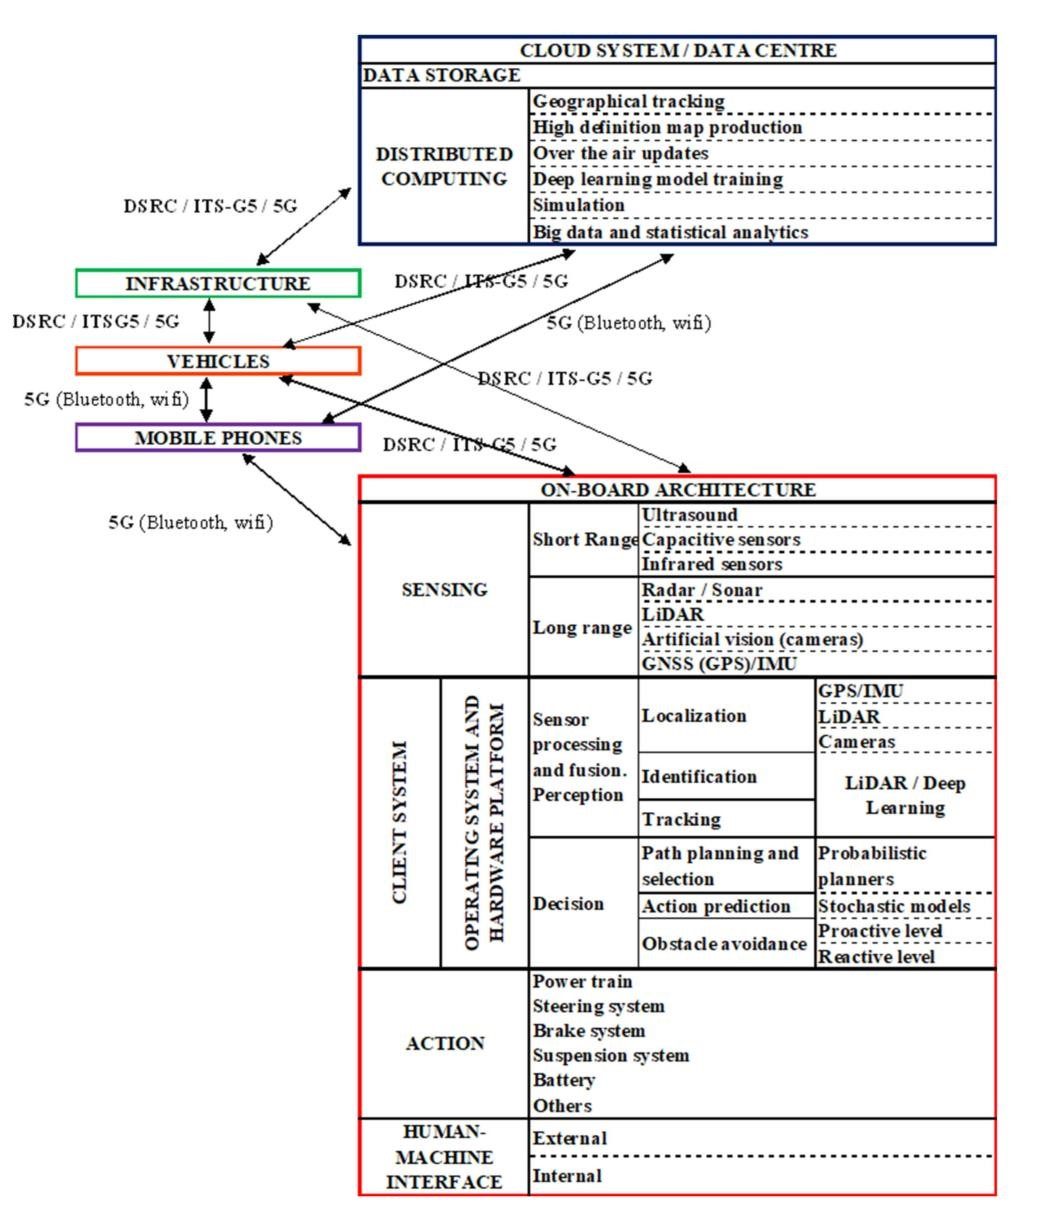
\includegraphics[]{assets/figures/Architektur.jpg}
	\begin{flushleft}
		Quelle: Martínez-Díaz, M./Soriguera, F./Pérez, I., Autonomous driving: a bird's eye view, 2019, S. 564.
	\end{flushleft}
\end{figure}

Stet clita kasd gubergren, no sea takimata sanctus est Lorem ipsum dolor sit amet Acceptance of autonomous driving will depend on how far a consensus on these norms can be found, first among experts, then in society at large.
One ethical condition, however, should be crucial: in no case should the ethical algorithms be put in practice as nontransparent black boxes.
The built-in norms should, as far as possible, be understood and commonly shared.

\section{Untersuchungsmethode}

Lorem ipsum dolor sit amet, consetetur sadipscing elitr, sed diam nonumy eirmod tempor invidunt ut labore et dolore magna aliquyam erat, sed diam voluptua.
At vero eos et accusam et justo duo dolores et ea rebum.
Stet clita kasd gubergren, no sea takimata sanctus est Lorem ipsum dolor sit amet.
Automation in cars has a long history.  Lorem ipsum dolor sit amet, consetetur sadipscing elitr, sed diam nonumy eirmod tempor invidunt ut labore et dolore magna aliquyam erat, sed diam voluptua.
At vero eos et accusam et justo duo dolores et ea rebum.\footnote{Vgl. Baumann, M. F. u. a., Taking responsibility: A responsible research and innovation (RRI) perspective on insurance issues of semi-autonomous driving, 2019, S. 558.}
Stet clita kasd gubergren, no sea takimata sanctus est Lorem ipsum dolor sit amet Acceptance of autonomous driving will depend on how far a consensus on these norms can be found, first among experts, then in society at large.
One ethical condition, however, should be crucial: in no case should the ethical algorithms be put in practice as nontransparent black boxes.
The built-in norms should, as far as possible, be understood and commonly shared.


\section{Literaturanalyse}

\begin{table}[h]
	\caption{Tolle Tabelle}
	\centering
	\begin{tabular}{ | c | c | c | }
		\hline
		cell1 & cell2 & cell3 \\
		cell4 & cell5 & cell6 \\
		cell7 & cell8 & cell9 \\
		\hline
	\end{tabular}
	\begin{flushleft}
		Quelle: Martínez-Díaz, M./Soriguera, F./Pérez, I., Autonomous driving: a bird's eye view, 2019, S. 564.
	\end{flushleft}
\end{table}

Lorem ipsum dolor sit amet, consetetur sadipscing elitr, sed diam nonumy eirmod tempor invidunt ut labore et dolore magna aliquyam erat, sed diam voluptua.
At vero eos et accusam et justo duo dolores et ea rebum.
Stet clita kasd gubergren, no sea takimata sanctus est Lorem ipsum dolor sit amet.
Automation in cars has a long history.  Lorem ipsum dolor sit amet, consetetur sadipscing elitr, sed diam nonumy eirmod tempor invidunt ut labore et dolore magna aliquyam erat, sed diam voluptua.
At vero eos et accusam et justo duo dolores et ea rebum.\footnote{Vgl. Baumann, M. F. u. a., Taking responsibility: A responsible research and innovation (RRI) perspective on insurance issues of semi-autonomous driving, 2019, S. 558.}
Stet clita kasd gubergren, no sea takimata sanctus est Lorem ipsum dolor sit amet Acceptance of autonomous driving will depend on how far a consensus on these norms can be found, first among experts, then in society at large.
One ethical condition, however, should be crucial: in no case should the ethical algorithms be put in practice as nontransparent black boxes.
The built-in norms should, as far as possible, be understood and commonly shared.

\section{Diskussion}

Lorem ipsum dolor sit amet, consetetur sadipscing elitr, sed diam nonumy eirmod tempor invidunt ut labore et dolore magna aliquyam erat, sed diam voluptua.
At vero eos et accusam et justo duo dolores et ea rebum.\footnote{Vgl. Baumann, M. F. u. a., Taking responsibility: A responsible research and innovation (RRI) perspective on insurance issues of semi-autonomous driving, 2019, S. 558.}
Stet clita kasd gubergren, no sea takimata sanctus est Lorem ipsum dolor sit amet.
Automation in cars has a long history.  Lorem ipsum dolor sit amet, consetetur sadipscing elitr, sed diam nonumy eirmod tempor invidunt ut labore et dolore magna aliquyam erat, sed diam voluptua.
At vero eos et accusam et justo duo dolores et ea rebum.
Stet clita kasd gubergren, no sea takimata sanctus est Lorem ipsum dolor sit amet Acceptance of autonomous driving will depend on how far a consensus on these norms can be found, first among experts, then in society at large.
One ethical condition, however, should be crucial: in no case should the ethical algorithms be put in practice as nontransparent black boxes.
The built-in norms should, as far as possible, be understood and commonly shared.

\subsection{Diskussion der These an Hand der Literatur}

Lorem ipsum dolor sit amet, consetetur sadipscing elitr, sed diam nonumy eirmod tempor invidunt ut labore et dolore magna aliquyam erat, sed diam voluptua.
At vero eos et accusam et justo duo dolores et ea rebum.\footnote{Vgl. Baumann, M. F. u. a., Taking responsibility: A responsible research and innovation (RRI) perspective on insurance issues of semi-autonomous driving, 2019, S. 558.}
Stet clita kasd gubergren, no sea takimata sanctus est Lorem ipsum dolor sit amet.
Automation in cars has a long history.  Lorem ipsum dolor sit amet, consetetur sadipscing elitr, sed diam nonumy eirmod tempor invidunt ut labore et dolore magna aliquyam erat, sed diam voluptua.
At vero eos et accusam et justo duo dolores et ea rebum.
Stet clita kasd gubergren, no sea takimata sanctus est Lorem ipsum dolor sit amet Acceptance of autonomous driving will depend on how far a consensus on these norms can be found, first among experts, then in society at large.
One ethical condition, however, should be crucial: in no case should the ethical algorithms be put in practice as nontransparent black boxes.
The built-in norms should, as far as possible, be understood and commonly shared.

\subsection{Qualität der Aussage}

Lorem ipsum dolor sit amet, consetetur sadipscing elitr, sed diam nonumy eirmod tempor invidunt ut labore et dolore magna aliquyam erat, sed diam voluptua.
At vero eos et accusam et justo duo dolores et ea rebum.
Stet clita kasd gubergren, no sea takimata sanctus est Lorem ipsum dolor sit amet.
Automation in cars has a long history.  Lorem ipsum dolor sit amet, consetetur sadipscing elitr, sed diam nonumy eirmod tempor invidunt ut labore et dolore magna aliquyam erat, sed diam voluptua.
At vero eos et accusam et justo duo dolores et ea rebum.\footnote{Vgl. Baumann, M. F. u. a., Taking responsibility: A responsible research and innovation (RRI) perspective on insurance issues of semi-autonomous driving, 2019, S. 558.}
Stet clita kasd gubergren, no sea takimata sanctus est Lorem ipsum dolor sit amet Acceptance of autonomous driving will depend on how far a consensus on these norms can be found, first among experts, then in society at large.
One ethical condition, however, should be crucial: in no case should the ethical algorithms be put in practice as nontransparent black boxes.
The built-in norms should, as far as possible, be understood and commonly shared.

\section{Fazit – Konsequnzen}

Lorem ipsum dolor sit amet, consetetur sadipscing elitr\footnote{Vgl. Baumann, M. F. u. a., Taking responsibility: A responsible research and innovation (RRI) perspective on insurance issues of semi-autonomous driving, 2019, S. 558.}, sed diam nonumy eirmod tempor invidunt ut labore et dolore magna aliquyam erat, sed diam voluptua.
At vero eos et accusam et justo duo dolores et ea rebum.
Stet clita kasd gubergren, no sea takimata sanctus est Lorem ipsum dolor sit amet.
Automation in cars has a long history.  Lorem ipsum dolor sit amet, consetetur sadipscing elitr, sed diam nonumy eirmod tempor invidunt ut labore et dolore magna aliquyam erat, sed diam voluptua.
At vero eos et accusam et justo duo dolores et ea rebum.
Stet clita kasd gubergren, no sea takimata sanctus est Lorem ipsum dolor sit amet Acceptance of autonomous driving will depend on how far a consensus on these norms can be found, first among experts, then in society at large.
One ethical condition, however, should be crucial: in no case should the ethical algorithms be put in practice as nontransparent black boxes.
The built-in norms should, as far as possible, be understood and commonly shared.

\chapter{Schluss}

Lorem ipsum dolor sit amet\footnote{Vgl. Baumann, M. F. u. a., Taking responsibility: A responsible research and innovation (RRI) perspective on insurance issues of semi-autonomous driving, 2019, S. 558.}, consetetur sadipscing elitr, sed diam nonumy eirmod tempor invidunt ut labore et dolore magna aliquyam erat, sed diam voluptua.
At vero eos et accusam et justo duo dolores et ea rebum.
Stet clita kasd gubergren, no sea takimata sanctus est Lorem ipsum dolor sit amet.
Automation in cars has a long history.  Lorem ipsum dolor sit amet, consetetur sadipscing elitr, sed diam nonumy eirmod tempor invidunt ut labore et dolore magna aliquyam erat, sed diam voluptua.
At vero eos et accusam et justo duo dolores et ea rebum.
Stet clita kasd gubergren, no sea takimata sanctus est Lorem ipsum dolor sit amet Acceptance of autonomous driving will depend on how far a consensus on these norms can be found, first among experts, then in society at large.
One ethical condition, however, should be crucial: in no case should the ethical algorithms be put in practice as nontransparent black boxes.
The built-in norms should, as far as possible, be understood and commonly shared.

\section{Kurzzusammenfassung der Arbeit}

Lorem ipsum dolor sit amet, consetetur sadipscing elitr, sed diam nonumy eirmod tempor invidunt ut labore et dolore magna aliquyam erat, sed diam voluptua.
At vero eos et accusam et justo duo dolores et ea rebum.
Stet clita kasd gubergren, no sea takimata sanctus est Lorem ipsum dolor sit amet.
Automation in cars has a long history.  Lorem ipsum dolor sit amet, consetetur sadipscing elitr, sed diam nonumy eirmod tempor\footnote{Vgl. Baumann, M. F. u. a., Taking responsibility: A responsible research and innovation (RRI) perspective on insurance issues of semi-autonomous driving, 2019, S. 558.} invidunt ut labore et dolore magna aliquyam erat, sed diam voluptua.
At vero eos et accusam et justo duo dolores et ea rebum.
Stet clita kasd gubergren, no sea takimata sanctus est Lorem ipsum dolor sit amet Acceptance of autonomous driving will depend on how far a consensus on these norms can be found, first among experts, then in society at large.
One ethical condition, however, should be crucial: in no case should the ethical algorithms be put in practice as nontransparent black boxes.
The built-in norms should, as far as possible, be understood and commonly shared.

\section{Weitere Empfehlungen}

Lorem ipsum dolor sit amet, consetetur sadipscing elitr, sed diam nonumy eirmod tempor invidunt ut labore et dolore magna aliquyam erat, sed diam voluptua.
At vero eos et accusam et justo duo dolores et ea rebum.
Stet clita kasd gubergren, no sea takimata sanctus est Lorem ipsum dolor sit amet.
Automation in cars has a long history.  Lorem ipsum dolor sit amet, consetetur sadipscing elitr, sed diam nonumy eirmod tempor invidunt ut labore et dolore magna aliquyam erat, sed diam voluptua.
At vero eos et accusam et justo duo dolores et ea rebum.
Stet clita kasd gubergren, no sea takimata sanctus est Lorem ipsum dolor sit amet Acceptance of autonomous driving will depend on how far a consensus on these norms can be found, first among experts, then in society at large\footnote{Vgl. Baumann, M. F. u. a., Taking responsibility: A responsible research and innovation (RRI) perspective on insurance issues of semi-autonomous driving, 2019, S. 558.}.
One ethical condition, however, should be crucial: in no case should the ethical algorithms be put in practice as nontransparent black boxes.
The built-in norms should, as far as possible, be understood and commonly shared.


%end

%end of document
\end{document}
